\chapter{Sistemas de recomendação}
\label{cap:sistemas_de_recomendacao}

% Introdução

% Falar sobre as mudança das coisas ligadas por "links" para por dados.

A web tem proporcionado diversas formas de interação, seja entre usuários ou entre sistemas e como resultado, tem-se uma grande quantidade de dados gerada. Os usuários que lidam com esses dados brutos certamente terão dificuldades em assimilar alguma informação útil e de seu interesse. É necessário, portanto, um modo de processar tal montante de dados e extrair informações úteis. 
% Contextualizar com a Amazon, Netflix entre outros

No contexto da IoT, os dispositivos conectados geram uma grande quantidade de dados brutos provenientes de sensores, câmeras, atuadores etc.

% Os Sistemas de Recomendação surgem como potencial solução para esse problema. Um Sistema de Recomendação (SR) a partir de dados coletados sobre seus usuários na forma de preferências em certos conjuntos de itens, ou seja, produtos, eventos, ações entre outros e outras fontes de informação, provê aos usuários previsões e recomendações de itens de acordo c.

Por baixo dos panos existe um Sistema de Recomendação (SR) no qual é capaz de analisar o perfil de cada usuário e, com base neste, fornecer recomendações de itens que possam lhe interessar. Os itens recomendados podem ser descritos como objetos, conselhos como filmes, livros, receitas, páginas web entre outros \cite{Bobadilla_2013}.

\section{Histórico}

A web primordial ou Web 1.0 era estática, na qual a única perspectiva de interação era o consumo de conteúdo, ou seja, apenas leitura deste se fazia possível. Era, portanto, amplamente utilizada por organizações na divulgação de seus produtos e serviços \cite{Aghaei2012}. 

% Falar sobre a web 2.0, e interação do usuário.
A Web 2.0, por outro lado, agregou dinamicidade à Internet a partir da viabilização da interação entre usuários e possibilidade de inserção de conteúdo na rede por parte desses, a partir de blogs e redes sociais, por exemplo \cite{Nath2014}.

% Falar da web 3.0
Com a Web 3.0, se deu a transformação da Web de Documentos presente nas versões anteriores para a Web de Dados, onde os diversos conteúdos deixam de se relacionar por links e passam a ser por dados e, assim, podem ser utilizados não apenas por usuários, mas por máquinas
%, às quais, usam a rede para acessar recursos externos entre outros.  
A Web 3.0 acrescentou, dessa forma, a possibilidade da comunicação entre dispositivos, além do aprimoramento do gerenciamento dos dados. 

A Web 3.0, é extendida pela Web Semântica, onde se propõe estender os princípios da web de documentos para a web de dados \cite{Nath2014}. 
A web de documentos consiste em objetos, como websites, e as ligações entre eles, isto é, os \textit{links}, com foco no consumo de conteúdo por pessoas. A web de dados, entretanto, torna legível o conteúdo da web para as máquinas, priorizando estas em detrimento dos humanos a partir da representação e organização das dados formato organizado como o \textit{Resource Description Framework} (RDF) \cite{Aghaei2012}.

Já se discute a cerca da Web 4.0, apesar de, conceitualmente, não bem definida. Propõe-se que, no futuro, haveria uma simbiose entre os computadores e as pessoas e, a partir disso, seria possível a construção de interfaces mais poderosas, como as controladas pela mente \cite{Aghaei2012}.

A ideia de fazer uso de todo o volume de dados gerados por muitos usuários, com a Web 2.0, para auxiliar na procura por conteúdos mais úteis e interessantes já existia desde a década de 1990 \cite{Jannach2010}.

%    PARC Tapestry system
O primeiro SR a introduzir o conceito de filtragem colaborativa, o PARC Tapestry System, foi um sistema experimental de e-mail desenvolvimento, ao qual objetivava categorizar o grande volume de e-mails recebidos em categorias de acordo com o interesse do usuário \cite{Goldberg1992}.
%    GroupLens - notícias
Alguns anos mais tarde, o \textit{GoodNews} foi desenvolvimento com o foco em notícias, onde cada artigo era avaliado de acordo com a média de avaliações do usuário e os melhores eram recomendados . Dessa forma, o sistema não levava em conta gostos de cada usuário e eliminava, assim, a necessidade de armazenamento de dados de usuários.
% Ringo system - filtragem colaborativa para músicas
Outro sistema desenvolvimento foi o Ringo, ao qual provia recomendações aos seus usuários a cerca de músicas. Inicialmente o usuário fornecia avaliações de cerca de 125 artistas e, de acordo com as respostas será feito uma avaliação do perfil do usuário.  A aplicação, então, passava a recomendar novos artistas e álbuns que o usuário poderia gostar \cite{Resnick1994}.

% Comercialização (...)
% Pesquisa (quais as pesquisar mais recentes
% Hoje (no que é usado, com qual finalidade);
% Definir item

Caracterizar

Falar sobre avaliações explícitas e implícitas

% Introduzir as abordagens e o que as diferencia

\section{Filtragem Colaborativa (FC)}
    
    Em diversas ocasiões do cotidiano as pessoas requisitam opiniões de outras a cerca de certos produtos ou serviços, seja filmes, restaurantes, equipamentos eletrônicos entre outros. A opinião do indivíduo, então, influencia na escolha do outro e o ajuda a tomar uma decisão sobre o problema. Por outro lado, uma pessoa próxima, um amigo, recomenda que assista a um certo filme de ação em cartaz nos cinemas, sabendo que a pessoa ainda não assistiu-o e que gosta de filmes do gênero. Esse indivíduo, portanto, certamente levará em conta o conselho, assistirá o filme, provavelmente gostará dele e recomendará a um outro amigo que também não viu o filme.    
    Com base nesse contexto de recomendações entre indivíduos, tem-se o conceito de Filtragem Colaborativa (FC), no qual, a partir de um perfil de preferências de um certo indivíduo, obtido através de seu histórico, em conjunto com as opiniões de outros usuários semelhantes a ele, prevê quais os itens que tem a maior possibilidade de gostar ou de se interessar \cite{Jannach2010}.

    % Explicação do conceito: qual a ideia, objetivos, vantagens e desvantagens.
        % Características
        % Não precisa das características específicas dos itens.

    % Não precisa das características específicas dos itens.
    % processamento custoso
        % Escalabilidade comprometida
    % maior precisão

    %"Se usuários compartilham interesses, eles terão gostos parecidos no futuro".
    %Pegar recomendações apenas dos melhores match's.
    
    Os sistemas baseados em filtragem colaborativa se utilizam da matriz de avaliações de itens pelos usuários, como mostrado na Tabela \ref{tab:matriz-av-item-user}, tendo esta como entrada. Como saída, gera-se previsões de avaliações que usuários aplicariam para itens por eles não avaliados ou um conjunto de melhores itens para recomendação. A partir do conjunto de dados da matriz é possível fazer uso de algoritmos que levem em conta as avaliações de todo o conjunto de usuários, para então definir qual é a avaliação plausível para um determinado item ou quais itens recomendar ao usuário \cite{Bobadilla_2013}.
    
    
    \begin{table}[htb]
        \centering
        \caption{Matriz de avaliações de itens por usuários}
        \label{tab:matriz-av-item-user}
        \begin{tabular}{@{}lcccccc@{}}
        \toprule
                  & Item 1 & Item 2 & Item 3 & Item 4 & Item 5 & Item 6 \\ \midrule
        Jack      & 5      & 4      & 2      & ?      & 5      & 1      \\
        Will      & 3      & 5      & 3      & 5      & 1      & 1      \\
        Elizabeth & 5      & 3      & 3      & 4      & 2      & 4      \\
        Hector    & 3      & 5      & 4      & 5      & 4      & 4      \\ \bottomrule
        \end{tabular}
    \end{table}
    
    Segundo \citeonline{Ricci2010}, os métodos de filtragem colaborativa podem ser classificados em duas classes: os baseados em memória ou em vizinhança e os métodos baseados em modelo. A principal diferença entre as abordagens está no modo de uso da matriz de avaliações na geração de recomendações. 
    
    % Não precisa das características específicas dos itens.
    
    % Ideia
    % para cada fórmula, um exemplo
    % ex: quando mostrar o pearson, calcular a similaridade entre dois usuários.
        
    \subsection{Baseado em memória}
        % processamento custoso
        % Escalabilidade comprometida
        % maior precisão
        
        % Usam diretamente os dados da matriz
        Métodos de recomendação baseados em memória operam diretamente sobre a base de dados de avaliações de itens pelos usuários. Além disso, as recomendações estarão sempre atualizadas devido ao uso das mais recentes avaliações recebidas dos usuários \cite{Bobadilla_2013}. 
        
        % Rever
        %No entanto, para grandes bases de dados onde existem milhares de itens a serem avaliados e milhares de usuários, os métodos baseados em memória são lentos em termos de processamento, dificultando o seu uso em recomendações geradas em tempo real \cite{Mustafa2017}.
        
        Em geral, os sistemas produzem recomendações com base no conceito de vizinho mais próximos, onde o objetivo é encontrar semelhanças entre usuários ou entre itens com suporte nas diversas avaliações adquiridas pela base de dados \cite{Mustafa2017}. Por exemplo, se um usuário tem preferência em certos filmes de ficção científica e existe um outro que também tem algum gosto pelo gênero, ambos poderão ser classificados como vizinhos próximos. Em casos como esse, o grau de semelhança é obtido a partir de cálculos de similaridade.
        
        \subsubsection{Similaridade}    
        
        % Definição
        A similaridade entre usuários, itens, etc., podem ser obtidas a partir da matriz de avaliações dos usuários em relação ao itens (citar).  
        Os diversos algoritmos operam sobre pares de linhas ou colunas da tabela para encontrar um valor numérico que caracterize o grau de afinidade entre os objetos da comparação. Além disso, uma abordagem geométrica pode ser utilizada para aprimorar a observação do comportamento desses algoritmos \cite{Jones1987}.
        
        % \subsubsection{Correlação de Pearson}
        O grau de semelhança entre dois usuários pode ser mensurado a partir de sua correlação, na qual estima a relação linear entre ambos. Dentre os diversos métodos, a correlação de \textit{Pearson} avalia vetores de mesma dimensão \cite{Ricci2010}. Considerando, um conjunto de produtos $P=\{p_1, p_2, ..., p_n\}$, um conjunto de usuários $U = \{u_1, u_2, ..., u_m\}$ e uma matriz de avaliações $R=\{r_{1,1}, r_{1,2}, ..., r_{n, m}\}$ desses produtos em função dos usuários, com dimensão  $n\times m$, tem-se a Equação \ref{eq:correlacao-pearson} que descreve a correlação de Pearson entre dois usuários $a$ e $b$.
             
        \begin{equation}
             % sim(a, b) =  \frac{\sum\limits_{i=1}^{n}(a_i-\bar{a})(b_i-\bar{b})}{\sqrt{\sum\limits_{k=1}^{n}(%a_k-\bar{a})^2}*\sqrt{\sum\limits_{j=1}^{n}(b_j-\bar{b})^2}} \label{eq:correlacao-pearson}
             sim(a, b) = \frac{\sum_{p\in P}(r_{a, p}-\bar{r_a})(r_{b, p}-\bar{r_b})}{\sqrt{\sum_{p\in P}(r_{a, p}-\bar{r_a})^2}\sqrt{\sum_{p\in P}(r_{b, p}-\bar{r_b})^2}}\label{eq:correlacao-pearson}
        \end{equation}
        
         Observa-se, inicialmente, a subtração de cada posição pelo valor médio das avaliações, o que reduz o efeito negativo, no cálculo, das no de um determinado usuários que, em sua maioria, são ou altas, ou baixas. Além disso, tem-se um produto interno como numerador e a multiplicação dos comprimentos como denominador. Como possíveis resultados, a correção de Pearson gera valores entre $-1$ a $1$, onde o primeiro indica correlação negativa perfeita, ou seja, usuários com preferências opostas, e o segundo demonstra correlação positiva perfeita, implicando em gostos equivalentes entre os usuários \cite{Jannach2010}.
        
        %Pearson: É melhor entre outras técnicas para comparar usuários
        
        Como exemplo, considerando a Tabela \ref{tab:matriz-av-item-user}, deseja-se encontrar a similaridade entre os usuários Will e Elizabeth a partir de suas respectivas avaliações para os seis (6) itens e a correlação de Pearson. Fazendo uso da Equação \ref{eq:correlacao-pearson}, tem-se o seguinte cálculo:
        
        \begin{eqnarray}
            sim(W, E) &=& \text{\footnotesize   $\frac{(3-3)(5-3,5)+(5-3)(3-3,5)+...}{\sqrt{(3-3)^2+(5-3)^2+...}\sqrt{(5-3,5)^2+(3-3,5)^2+...}} $} \nonumber \\
            sim(W, E) &=& 0,21 \nonumber
        \end{eqnarray}
    
        Os usuários Will e Elizabeth têm portanto uma similaridade medida pela correlação de Pearson de $0,21$ indicando que ambos têm alguma semelhança entre suas preferências.
    
        %##########    Cosseno    ###################
        Em relação a similaridade de itens, o método do \textit{cosseno} é considerado o padrão. Como base para o seu cálculo se faz uso das avaliações dadas por todos os usuários a cada item, ou seja, as colunas da matriz de avaliação são utilizadas. No entanto, o método do cosseno não leva em conta o perfil de cada usuário ao considerar apenas a avaliação dada ao item em questão\cite{Jannach2010}.
        
        A Equação \ref{eq:sim-cosseno} define o cálculo de similaridade pelo método do cosseno onde, calcula-se o produto interno entre os vetores de avaliações dos itens, como numerador e a multiplicação dos comprimentos L2 de cada um como denominador.         
        
        %cosseno: É melhor que Pearson para comparar itens.
        %Jones
        \begin{equation} 
            sim(a, b) = \frac{\sum_{u\in U}(r_{u, a})(r_{u, b})}{\sqrt{\sum_{u\in U}(r_{u, a})^2}\sqrt{\sum_{u\in U}(r_{u, b})^2}} \label{eq:sim-cosseno}
        \end{equation}    
    
        Em outras palavras, para cada usuário $u$ pertencente ao conjunto de usuário $U$, é calculada a multiplicação das suas avaliações para cada item e somada aos demais resultados da operação e, por fim, calcula-se o módulo de cada vetor. Um outra interpretação para o cálculo é considerar como sendo o produto interno entre os vetores de avaliação normalizados \cite{Jones1987}. Assim, com a divisão pelo comprimento, os possíveis resultados permanecem entre $0$ e $1$ \cite{Jannach2010}, sendo que geometricamente, esses resultados podem ser avaliados como ângulos. As avaliações de um item podem ser consideradas componentes de um vetor que representa o objeto. Inserindo, então, os vetores num plano será formado um ângulo $\theta$ no qual, no contexto das avaliações de itens é obtido partir do arco cosseno do resultado da similaridade. Quanto mais próximo, esse ângulo estiver de zero grau ($0^o$), maior será a semelhança entre os itens.
        
        Como exemplo, pretende-se encontrar o grau de similaridade entre Item 2 e Item 5. Para tanto, considera-se as respectivas colunas de avaliações que usuários forneceram à cada um e a Equação \ref{eq:sim-cosseno}. Por fim, tem-se o seguinte cálculo:
        
        \begin{eqnarray}
            sim(2, 5) &=& \frac{(4\cdot 5)+(5\cdot 1)+(3\cdot 2)+(5 \cdot 4)}{\sqrt{4^2+5^2+3^2+5^2}\sqrt{5^2+1^2+2^2+4^2}} \nonumber \\
            sim(2, 5) &=& 0,87 \nonumber
        \end{eqnarray}
        
        Os itens 2 e 5, portanto tem alta similaridade. Além disso, ao considerar a visão geométrica, têm-se um ângulo de $29,5^o$ formado entre os itens.
    
        %##########    Cosseno ajustado   ###################
        Como dito anteriormente, o método do cosseno não leva em conta o perfil de avaliações do usuário no cálculo da similaridade entre itens, no entanto, um método semelhante a ele chamado \textit{cosseno ajustado}, que como o nome deixa claro, é uma alteração do método original. Primeiramente, define-se o cálculo pela Equação \ref{eq:sim-cosseno-ajustado}.
        
        \begin{equation}
             sim(a, b) = \frac{\sum_{u\in U}(r_{u, a}-\overline{r_u})(r_{u, b}-\overline{r_u})}{\sqrt{\sum_{u\in U}(r_{u, a}-\overline{r_u})^2}\sqrt{\sum_{u\in U}(r_{u, b}-\overline{r_u})^2}} \label{eq:sim-cosseno-ajustado}
        \end{equation}
        
        Observa-se, então, que o ajuste se refere à subtração da média das avaliações dadas pelo usuário $u$ a todos os itens. Assim, o efeito negativo causado pela média alta ou baixa de avaliações do usuário é reduzido, deslocando as avaliações para a média do usuário ao invés da média do item. Além disso, o intervalo de valores possíveis com o método do cosseno ajustado, diferentemente do cosseno, é de $-1$ a $1$ \cite{Jannach2010, Ricci2010}. Por outro lado, nota-se a semelhança do método do cosseno ajustado em relação à correlação de Pearson, descrita na Equação \ref{eq:correlacao-pearson}, no entanto, apesar de semelhantes, os contextos aos quais aplica-se cada método é diferente. A correlação de Pearson é utilizada para o cálculo de similaridade entre usuários, já o cosseno ajustado destina-se a encontrar a semelhança entre itens, apesar de ambas fazerem uso da média de avaliações de cada usuário.
        
        %
        \subsubsection{k Vizinhos Mais Próximos (kNN)}
            
            O kNN é um dos principais algoritmos para geração de recomendação e previsões de avaliações \cite{Bobadilla_2013}. Originalmente, foi implementado com o intuito de operar um classificador. Assim, dado um ponto em um espaço, o kNN encontrará os k pontos mais próximos com base em um conjunto de outros pontos pré-classificados . Como exemplo, a \reffig{cap3_knn-no-class} traz dois conjuntos de pontos, azuis mais abaixo na imagem e vermelhos acima. Em meio a esses pontos à um outro, rosa, ao qual deseja-se saber à qual grupo pertence (independentemente de sua cor).             
            
            \begin{figure}[htb]
                \caption{Exemplo de grupos para classificação com o kNN}
                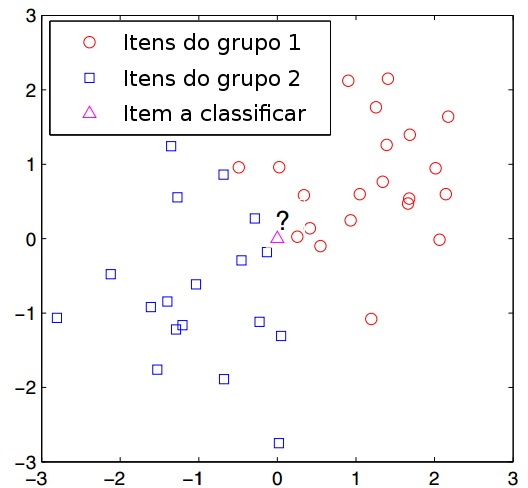
\includegraphics[width=0.55\textwidth]{cap3_knn-no-class}
                \label{fig:cap3_knn-no-class}
                
                {\footnotesize Fonte: Adaptado de \citeonline{Ricci2010}}
            \end{figure}
                        
            A partir de cálculos de similaridade o algoritmo encontrará os $k$ pontos mais próximos, onde tal valor varia de acordo o contexto da aplicação. \citeonline{Duda2000} sugerem um $k$  igual a raiz quadrada do total de pontos $n$, ou seja, $k$ é igual $\sqrt{n}$, no âmbito geral de classificadores, já no contexto de sistemas de recomendação, \citeonline{Jannach2010} afirma que $k$  entre $20$ a $50$ é uma boa estimativa. 
            
            Em um aspecto gráfico, $k$ pode ser interpretado como o número de pontos aos quais podem ser inseridos dentro de um círculo centrado no ponto que será classificado, como pode ser visualizado na Figura \reffig{cap3_knn-class}. 
            
            \begin{figure}[htb]
                \caption{Exemplo de classificação com o kNN}
                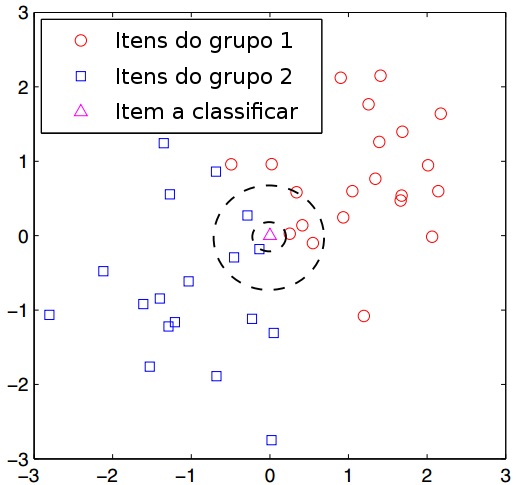
\includegraphics[width=0.55\textwidth]{cap3_knn-class}
                \label{fig:cap3_knn-class}
                
                {\footnotesize Fonte: Adaptado de \citeonline{Ricci2010}}
            \end{figure}            
            
            % CF baseado em kNN é simples e implementação direta
                 
            O algoritmo de $k$ vizinhos mais próximos opera em três etapas, sendo a primeira, a determinação dos vizinhos mais próximos do usuário $x$ conforme cálculos de similaridade. A seguir, previsões são computadas sobre as avaliações que $x$ daria a itens, aos quais, ainda não conhece, a partir de funções de agregação como, por exemplo, média e soma ponderada de notas de outros usuários ao item. Por fim, com nas avaliações obtidas, os $m$ melhores itens são recomendados ao usuário. \cite{Bobadilla_2013}.
            
                
            %     
            %\subsubsection{FC baseada em usuário}
                            
            % mais custosa (online), toda vez que for recomendar, tem que calcular tudo de novo.
            % encontrar usuários semelhantes com 
            % Baseado em item
          %  \subsubsection{FC baseada em item}
            % compara os itens com base nas avaliações dos usuários. 
            % "Quem gosta desse item também costuma gostar deste".
            % Menos custos (offline)
    
    
    \subsection{Baseado em modelo}
    % processamento offline
    
        
        \subsubsection{Fatoração de matriz}
        abc
        
        \subsubsection{Probabilístico}
        abc
        
        \subsubsection{Redes Neurais}
        
        abc
        \subsubsection{Baseado em regras}
        

    
\section{Baseada em conteúdo}
acbc
        
\section{Híbrida}
    abc
    % Aproveita o melhor de cada abordagem e 
    
\section{Baseada em conhecimento}
    acb
    
\section{Outras Abordagens}
    % Baseado em contexto
    
% Estudar também a questão geográfica (recomendação de acordo com o lugar) porque no caso de comida, as comidas mais apropriadas para cada indivíduo estão imersas num contexto cultural.
\section{Desafios}
     % Problemas: cold-start, esparçabilidade, escalabilidade, shilling attacks ... Soluções propostas por outros autores.
    
    Os sistemas de recomendação apresentam algumas limitações e obstáculos que dificultam que as recomendações sejam calculadas e realizadas. 
    
    Quando o sistema recebe novos usuários para recomendação não há informações suficientes sobre suas preferências que possibilite a geração de  recomendações para ele. Por outro lado, em relação aos itens, não existe nenhuma interação com usuários que permita ser recomendado a alguém. Os sistemas de recomendação ``puros'', ou seja baseados em filtragem colaborativa, baseados em conteúdo entre outros, não conseguem lidar com esses problemas, também chamados de \textit{cold start}, isto é partida fria, no entanto, sistemas híbridos o fazem \cite{Miranda2010}.
    
    Além do problema em recomendar novos itens, há o efeito gerado pela adição deste item, ou seja, o conjunto de recomendação prévio não leva em conta esse novo item e, portanto, pode não ser preciso. Assim, é necessário que o sistema ajuste as bases de recomendação para que o novo item seja recomendado. No entanto, tais bases contêm entre centenas à milhares de itens e usuários e, por isso, efetuar a atualização de uma base de grande porte pode ser custoso e inviável para cada novo item acrescentado. Esse problema se refere à \textit{escalabilidade} de sistemas de recomendação \cite{Lue2012}. 
    
    Outro desafio se refere a \textit{esparsabilidade}, ou seja, a proporção dos itens avaliados por usuários em relação ao número total de itens é consideravelmente pequena e mal distribuída. Além disso, a intersecção do conjunto de itens avaliados por pares de usuários tende a ser modesta. Isso acontece em função da baixa taxa de avaliação de itens, seja explícita ou implicitamente \cite{Lue2012}.

        % pode ser feito em parte offline

\section{Aplicações}

% Netflix Prize
% Spotify
% Financeiro
% IoT
% Turístico